%\section{The brain}
The \textbf{brain} is an exquisite piece of evidence for energy-efficient biological computation; the result of millions of years of an evolutionary process. It's been subject of multiple studies and, yet, we are barely getting to know it. The human brain consists of around $10^{12}$ \emph{neurons} which are interconnected through about $10^{15}$ special structures known as \emph{synapses}.
%It can perform the most diverse activities, from bird spotting to mathematics to art. All of this with about 20 watts of energy spread across many small computational units called \emph{neurons}.
\section{The Brain}
\label{sec:brain:brain}
The brain is an exquisite piece of biological computation

evolved from few neurons into the cortex

It consists of around 100 million neurons interconnected through 100 billion synapses

It can perform the most diverse tasks, from bird spotting to mathematics to music

All of this with high efficiency


\section{The hippocampus}
\label{sec:brain:hippo}
The hippocampus is a small organ with a seahorse-like shape that lies in the centre of the brain, right bellow the cortex (Figure~\ref{fig:brain:hippo}). It's part of the limbic system and it is thought to play a huge role in memory consolidation and spatial navigation.
The shape of the hippocampus is similar across mammals and its size increases with body size. There is also a relation between the size of the hippocampus and spatial memory. When compared in different species, the ones that present greater navigational abilities have larger hippocampi~\cite{jacobs2003evolution}. A similar phenomenon was found in humans, a study found that taxi drivers had an enlarged posterior section of the hippocampus when compared to the general public~\cite{taxi-maguire}.

\begin{figure}[h]
  \begin{center}
    \includegraphics[width=0.5\textwidth]{Gray739-emphasizing-hippocampus}
    \caption{The cyan blob at the lower end of the diagram is the hippocampus~\cite{wikipedia-images}. }
    \label{fig:brain:hippo}
  \end{center}
\end{figure}

Studies of moving rodents have found that hippocampal neurons have preference for spatial and navigational features~\cite{okeefe1971hippocampus,milford2010robot}:
\begin{description}
  \item[Place cells.] They emit bursts of action potentials whenever the animal passes through a location in their environment. The environment that makes a place cell to fire is called a place field. Nonetheless, place cells' firing is also affected by other factors (e.g. visual cues, food location).
  \item[Head direction cells.] These cells react profusely to a preferred direction of the rodent's head. The firing rate seems to be independent of body direction, though some cells may be influenced by the animal's velocity.
  \item[Grid cells.] Neurons in this group increase their firing rate when the rodent is located in the intersection of a grid-like representation of the environment.
  \item[Border cells.] If a border that is large enough to modify the path of the rodent is present, this type of neurons will fire continuously.
\end{description}

\begin{figure}[h]
  \begin{center}
    \includegraphics[width=0.7\textwidth]{cell_types_tuning1}
    \caption{Different hippocampal neuron's response to their preferred stimulus (adapted from~\cite{kloosterman-images}.)}
  \end{center}
\end{figure}

In primates, head direction cells' firing rate depends on direction of the head but not the direction of the eyes. Other work on primates, states that some hippocampal cells actually react to where the animal is looking, these are known as \emph{spatial view cells}~\cite{rolls2006spatial}. This evidence suggests that, one of the functions of the hippocampus might be to act as a cognitive map of the environment. 

%Episodic memories for nav
\section{Neurons and responses}
\label{sec:brain:neurons}
Neurons are small cells composed of a soma (body), dendritic and axonal tree for communication

Theories suggest they perform some kind of calculation, most of the time modelled as a threshold activation function

Latest evidence suggests that they communicate through spikes, on-off responses


\subsection{Neuron models}

Mathematical models for the membrane potential behaviour started appearing in the early 1900 CE. They range from the extremely detailed ones that consist of several differential equations to simple ones with just one or two and they all model the electrical properties of the nerve cells. 

A particular group of models (self-compartment) describes the neuron as an isopotential sphere, that is, all its surface has the same electrical potential (Figure~\ref{fig:neuro:isopotential})~\cite{dayan2001theoretical}.

\begin{figure}[hbt]
  \begin{center}
    
\includegraphics[width=0.45\textwidth]{iso_electrical_model}
    \caption{Diagram of the isopotential neuron. Adapted from \emph{Theoretical Neuroscience} by Dayan and Abbott~\cite{dayan2001theoretical}.}
    \label{fig:neuro:isopotential}
  \end{center}
\end{figure}

Since the neuron is modelled as a sphere, the membrane \emph{capacitance} $C_{m}$ and \emph{resistance} $R_{m}$ are specified in relation to its area $A$.

\begin{align}
R_{m} = r_{m}/A \\
C_{m} = c_{m}A
\end{align}
where $r_{m}$ and $c_{m}$ are the resistance and capacitance per unit area, 
respectively. Their values are $r_{m} \approx 1M \Omega mm^{2}$ and $c_{m} 
\approx 10nF/mm^{2}$. The basic relations of the electrical properties of the membrane are shown in  
Fig.~\ref{fig:neuro:isopotential}, are as follows:

\begin{align}
\Delta V &= I_{e}R_{m} \label{eq:neuro:volt-shift}\\[0.5em]
Q &= C_{m}V \label{eq:neuro:charge} \\[0.5em]
C_{m}\frac{dV}{dt} &= \frac{dQ}{dt} \label{eq:neuro:cap-curr}
\end{align}

When the membrane's potential changes, it does so according to Eq.~\ref{eq:neuro:volt-shift}. Variable $Q$ is the membrane's electrical charge which is proportional to its voltage and capacitance, as seen in Eq.~\ref{eq:neuro:charge}.
Currents originated by ion channels are thought to be linear, and can be modelled using Ohm's law
\begin{equation}
i_{x} = g_{x}(V - E_{x}) 
\label{eq:neuro:single-channel-curr}
\end{equation}
where $E_{x}$ is the \emph{reverse potential} due to ion exchange in channel $x$ and $g_{x}$ is the per unit area conductance of the channel. The total membrane current due to channels (per unit area) will be 
\begin{equation}
i_{m} = \sum_{x} i_{x} = \sum_{x} g_{x}(V - E_{x}) \label{eq:neuro:total-channel-curr}
\end{equation}

For the total membrane current due to ion channels Eq. \ref{eq:neuro:total-channel-curr} has to be multiplied by total area $A$.
The right hand side of Eq.~\ref{eq:neuro:cap-curr} is the total current in the membrane. Since we are adding an external current $I_{e}$ and is of opposite direction to $I_{m}$, the total current in the membrane is
\begin{equation}
I_{T} = I_{e} - I_{m} 
\label{eq:neuro:total-curr}
\end{equation}

Combining equations~\ref{eq:neuro:cap-curr}~and~\ref{eq:neuro:total-curr} gives the basic equation used by most self-compartment models~\cite{dayan2001theoretical}.
\begin{align}
C_{m} \frac{dV}{dt} &= I_{e} - I_{m} 
\label{eq:neuro:basic-self-compartment} \\[0.5em]
c_{m} \frac{dV}{dt} &= \frac{I_{e}}{A} - i_{m}
\label{eq:neuro:basic-pu-self-compartment}
\end{align}


\subsubsection{Leaky Integrate-and-fire}
This is one of the oldest neuron models, but it's still being used due to its simplicity. In the passive \emph{integrate-and-fire} all the membrane conductances are modelled by a single term $G_{L}$ (Equation~\ref{eq:neuro:passive-int-n-fire}).
\begin{equation}
C_{m}\frac{dV}{dt} = I_{e} - G_{L}\left( V - E_{L} \right) 
\label{eq:neuro:passive-int-n-fire}
\end{equation}
the rightmost term is also known as leak current. If Eq.~\ref{eq:neuro:passive-int-n-fire} is multiplied by the membrane resistance ($R_{m}$), we obtain
\begin{equation}
\tau_{m}\frac{dV}{dt} = R_{m}I_{e} - V + E_{L}  
\label{eq:neuro:passive-R-int-n-fire}
\end{equation}
Integrating Eq. \ref{eq:neuro:passive-R-int-n-fire} results in an expression for the voltage behaviour under non-spiking conditions.
\begin{equation}
V\left( t \right) = E_{L} + R_{m}I_{e} + 
                    \left( V\left( 0 \right) - E_{L} - R_{m}I_{e}\right) e^{ -t/\tau_{m}}
\label{eq:neuro:passive-V-int-n-fire}
\end{equation}
Spiking behaviour is added artificially once $V(t)$ reaches a certain threshold, afterwards it's reset back to $V(0)$.


\subsubsection{Hodgkin-Huxley}
In 1952, Hodgkin and Huxley published a paper that reflected their ground-breaking experimental work on the axon of the squid~\cite{hodgkin-huxley}. They found that the currents in the membrane are mainly due to changes in the concentration of three ions: potassium ($K^{+}$), sodium ($Na^{+}$) and chlorine ($Cl^{-}$). The first two are related to voltage dependant conductance and the last to a leak current. Under these considerations, Eq. \ref{eq:neuro:basic-self-compartment} becomes~\cite{dynamical-systems-Izhikevich2007}:
\begin{equation}
C_{m}\frac{dV}{dt} = I_{e} - g_{K}  n^{4} (V - E_{K}) 
                           - g_{Na} m^{3}h(V - E_{Na})
                           - g_{L}        (V - E_{L})
\label{eq:neuro:hodgkin-huxley}
\end{equation}
the variables $n$, $m$ and $h$ have the following behaviour
\begin{align}
\frac{dn}{dt} &= \alpha_{n}(V) (1 - n) - \beta_{n}(V) n \\[0.5em]
\frac{dn}{dt} &= \alpha_{m}(V) (1 - m) - \beta_{m}(V) m\\[0.5em]
\frac{dn}{dt} &= \alpha_{h}(V) (1 - h) - \beta_{h}(V) h
\end{align}
%and
%\begin{align}
%\alpha_{n}(V) &= 0.01\frac{10 - V}{e^{(10 - V)/10} - 1 } \qquad \qquad 
%\beta_{n}(V) = 0.125 e^{-V/80} \\[0.5em]
%%
%\alpha_{m}(V) &= 0.1\frac{25 - V}{e^{(25 - V)/10} - 1 } \qquad \qquad 
%\beta_{m}(V) = 4 e^{-V/18} \\[0.5em]
%%
%\alpha_{h}(V) &= 0.07\frac{10 - V}{e^{(10 - V)/10} - 1 } \qquad \qquad 
%\beta_{h}(V) = 0.125 e^{-V/80}
%\end{align}

The Hodgkin-Huxley model is one of the most detailed neural models so far, it's served as inspiration and foundation of many studies. The main issue with this level of detail is that it comes at a price, it's computationally expensive; so for system simulating a big number of neurons the hardware has to be equally powerful.

\subsubsection{Simple model}
The dynamics of the Hodgkin-Huxley were studied using bifurcation diagrams and approximated by \citeauthor{fitzhugh1961impulses}~\cite{fitzhugh1961impulses}. Using similar ideas and techniques, \citeauthor{izhikevich2003simple} developed what he named the \emph{simple model} of spiking neurons~\cite{izhikevich2003simple}. This model emulates the dynamics of membrane voltage on the sub-threshold area, for modelling the spike behaviour comes at the cost of tiny time-steps that increase the computational cost. \citeauthor{izhikevich2003simple}'s simple model consists of a pair of equations:
\begin{align}
  \frac{dv}{dt} &= 0.04v^{2} + 5v + 140 - u - I \\[0.5em]
  \frac{du}{dt} &= a(bv - u)
\end{align}
where $v$ represents membrane voltage and $u$ a negative feedback to $v$. The rising part of spiking behaviour is produced by the equations, though an artificial voltage reset is needed afterwards. When variable $v$ reaches 30 $mV$ or more, variables $v$ and $u$ are set as follows
\begin{equation}
  v = c \qquad u = u + d
\end{equation}
Parameters $a$, $b$, $c$ and $d$ are dimensionless and time has a $ms$ resolution~\cite{dynamical-systems-Izhikevich2007}. 

The simple model has, at least, two advantages: first, many observed neural behaviours can be replicated by modifying the model's parameters; and second, it keeps biological plausibility while having low computational cost~\cite{izhikevich2004model}. This model seems to be the right candidate for large-scale, biologically-plausible and energy-efficient systems.













\section{Different languages}
\label{sec:brain:codes}
In the previous sections, we discussed about the anatomy of the brain and neurons and how studies indicate that these cells might communicate via electrochemical pulses known as spikes. We know that sensory input is somehow encoded so that the brain can process it, the exact encoding is not yet known and is the subject of active research effort. Similarly, how is the brain able to reconstruct (or decode) prior input from action potentials is an open question. The so called \emph{neural code} is one of the most important questions in neuroscience and different hypotheses have been proposed, some of which are described bellow~\cite{dayan2001theoretical,gollisch2009throwing}.

\subsection{Rate code}
Spike-rate encoding, in its simplest case, represents information with the amount of action potentials that a neuron generated in a time interval. It is one of the earliest attempts of explaining neural encoding and gives a nice transition from traditional artificial neural networks to spiking ones. Furthermore, there's evidence that neurons that are in direct contact with sensory or motor organs encode information in this way (i.e. the stronger a muscle is flexed, the higher the rate of spikes generated by neurons near muscular tissue).

The main issue with this type of encoding is that it is unable to represent  a large array of different values. For example, if we have a time-slot of $10 ms$ and spikes last $1 ms$, we can only encode 10 values per neuron. Figure \ref{fig:neuro:spike-rate-encoding-cap} shows the case of a $1/10$ rate, no matter when the spike is fired, the encoded value would still be the same.

\begin{figure}[hbt]
  \begin{center}
    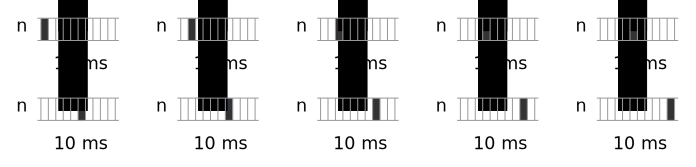
\includegraphics[width=0.8\textwidth]{spike_codes-rate-1}
    \caption{Spike rate example, all 10 combinations encode the same value for they all have a 1 spike per 10 $ms$ rate}
    \label{fig:neuro:spike-rate-encoding-cap}
  \end{center}
\end{figure}

\subsection{Rank-order}
Using this type of encoding, only the temporal order of the spikes generated by a group of neurons is important. It provides more information representation capacity and has been used in computer vision tasks~\cite{rank-order-sparse-memory,basab-model,thorpe-rate-coding-theory}.

\begin{figure}[hbt]
  \begin{center}
    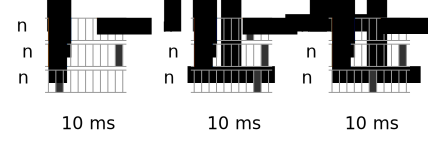
\includegraphics[width=0.55\textwidth]{spike_codes-rank}
    \caption{Rank-order example, since all the examples have neurons firing in the same order, they all encode the same value.}
    \label{fig:neuro:spike-rank-order}
  \end{center}
\end{figure}

An issue that has been noted by some on rank-order encoded information is the fact that spike trains that are notably different (Figure \ref{fig:neuro:spike-rank-order}) are interpreted as the same value. This might be corrected by changing the metrics used to determine the uniqueness of a spike train set~\cite{Cessac2010}. On the other hand, this same issue could be seen as a robust way of encoding information.

\subsection{Temporal code}
The precise time a spike was emitted encodes information. Lots of information, but still difficult to use. Polychronization might be the answer to learning/training.



Input from sensors is most likely rate-based, though processing time and energy consumption in the brain suggests a different one is used for further processing

\subsection{Latency}
\section{Conclusions}
The brain is an amazing organ, responsible for a broad range of tasks from allowing an animal to hunt to human culture. Simulating the brain or even a single task the brain does in a biologically plausible way is still subject of active research. For \emph{fast} vision tasks the combination of spiking neural networks using temporal codes looks like the optimal path to follow. Izhikevich's simple model of spiking neurons seems appropriate for its computation-efficiency to biological-fidelity ratio.